\chapter{Thick--Client VS. Web--Browser--based Software--System Architecture}

\vspace{-1em}

\YEROTHCHAPINTRO{
This comparison chapter tabular evaluates why
\thickclient are BETTER THAN \webbrowserbased
software--system architectures !
}

\vspace{1em}

\section{Thick--client: $2$ layers logical software architecture}

\begin{center}
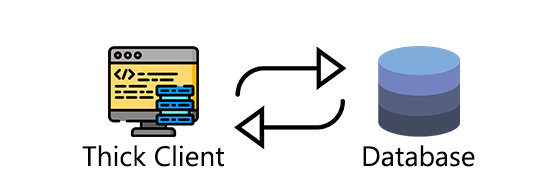
\includegraphics[scale=0.52]{images/yeroth-thickclient-application-two-tier-architecture.png}
\captionof{figure}{$2$--layers logical 
architecture of \thickclient software--system 
(Image copied from \cite{securityboulevarddotcom:2020}).}
\label{fig:yeroth-thickclient-application-two-tier-architecture}
\end{center}
\index{$2$--layers logical architecture of \thickclient software--system}

Figure~\ref{fig:yeroth-thickclient-application-two-tier-architecture}
illustrates an example of a \thickclient
software--system with a $2$--layers
logical architecture.


\section{Web--browser based: at least $4$ layers logical software architecture}

\begin{center}
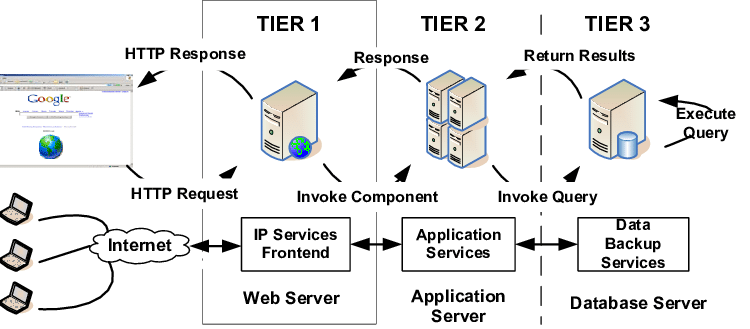
\includegraphics[scale=0.39]{images/yeroth-three-tier-architecture.png}
\captionof{figure}{$4$--layers logical architecture
of \webbrowserbased software--system
(Image copied from \cite{trevor:2006}).}
\label{fig:yeroth-three-tier-architecture}
\end{center}
\index{$4$--layers logical architecture of \webbrowserbased software--system}

Figure~\ref{fig:yeroth-three-tier-architecture}
illustrates an example of a \webbrowserbased
software--system with a $3$--layers
logical architecture.

Table~\ref{tab:thickclient-application-againts-webbrowserbased-application}
compares \thickclient software--systems against
\webbrowserbased software--systems.


\newpage


\section{A Tabular Comparison Between Thick-Client And Web Browser--based Architecture}
\index{comparison table between \thickclient and \webbrowserbased software--system}
\begin{table*}[!htbp]
\centering
\resizebox{\textwidth}{!}{%to fit the table within the text width
\begin{tabular}{cccc} 

\multicolumn{1}{c}{}										&
Thick--client application \mycheckmark{yerothColorBlue}	& 
Web--browser--based application								\\ \hline

business code								&
		\yerothvert{user interface}			&						
		\yerothrouge{application server}	\\ \hline
		
co--related software--systems		&
		\yerothvert{$1$ (DBMS)}		&						
		\yerothrouge{at least $3$ (DBMS, web~/~application server)}	\\ \hline
						
number of logical layers									&
		\yerothvert{$2$ (client and data)}					&						
		\yerothrouge{$4$ (client, presentation, logic, and data)}\\ \hline
				
rapid prototyping (\wy tools)		&
		\yerothvert{yes}			&						
		\yerothrouge{very limited}	\\ \hline				
				
software security vulnerability										&
		\yerothvert{low ($1$ programming language)}					&					
		\yerothrouge{high (\emph{several} programming languages)}	\\ \hline

user interface 														&
		\yerothvert{all computers (GUI with \emph{BUSINESS CODE})}	&						
		\yerothvert{all computers (web--browser)}					\\ 		


\end{tabular}}
\caption{Thick--client application VS Web--browser--based application.\\}
\label{tab:thickclient-application-againts-webbrowserbased-application}
\end{table*}

Table~\ref{tab:thickclient-application-againts-webbrowserbased-application}
illustrates the advantages of \thickclient
software--system architecture over \webbrowserbased
software--system architecture !
\newline

\textcolor{purplish}{
The common argument for \webbrowserbased software--system 
architecture is you update the business code just at $1$
place: \emph{the application server} !}

\textcolor{purplish}{
I argue that \thickclient architecture IS JUST AS WELL
BEST UPDATED AT $1$ PLACE: \emph{the user's computer}.}

\textcolor{purplish}{
The issue of automatic software upgrade in a computer
network is best solved by the 'apt upgrade software--system
of \debianlinux', as an example !
}